\documentclass{article}
% General document formatting
\usepackage[a4paper, total={5.5in, 7.5in}]{geometry}
\usepackage[parfill]{parskip}
\usepackage[utf8]{inputenc}
\usepackage{listings}
\usepackage{svg}
\usepackage{float}
\usepackage{caption} 

\usepackage{xcolor}
\usepackage[many]{tcolorbox}

% Caption font
\usepackage{titlesec}

\titleformat*{\section}{\Large\bfseries\sffamily}
\titleformat*{\subsection}{\large\bfseries\sffamily}
\titleformat*{\subsubsection}{\itshape\bfseries\sffamily}

\usepackage{etoolbox}
\apptocmd{\thebibliography}{\raggedright}{}{}

% Related to math
\usepackage{amsmath,amssymb,amsfonts,amsthm}

% % Referencing
\usepackage{hyperref}

\tcolorboxenvironment{lstlisting}{
  spartan,
  frame empty
  boxsep=0mm,
  left=1mm,right=1mm,top=-1mm,bottom=-1mm,
  colback=gray!45,
}

% spell-checker: disable %
\lstset{
    captionpos=b,
    commentstyle=\color{mygreen},
    basicstyle=\linespread{0.67}\ttfamily,
    aboveskip=2em,
    belowskip=1em,
}
\lstdefinestyle{bashStyle}{
    belowcaptionskip=1\baselineskip,
    breaklines=true,
    frame=none,
    numbers=none,
    basicstyle=\footnotesize\ttfamily,
    keywordstyle=\bfseries\color{green!40!black},
    commentstyle=\itshape\color{purple!40!black},
    identifierstyle=\color{blue},
}
% spell-checker: enable %


\begin{document}

\captionsetup{justification=centering}

\begin{titlepage}
    \begin{center}
        \vspace*{1cm}
 
        \textbf{Mini-Project MA-ICR}
 
        \vspace{0.5cm}
            A shared encrypted network file system
             
        \vspace{1.5cm}
 
        \textbf{Titus Abele}
 
        \vfill
             
        MSE Computer Science\\
        HES-SO Master\\
        Lausanne, Switzerland\\
        \today
             
    \end{center}
\end{titlepage}

\tableofcontents
\lstlistoflistings
\listoffigures

\section*{Repositories on GitHub}
\begin{itemize}
  \item The report is hosted on this repository: \href{https://github.com/TitusVM/icr/tree/main/06-mp}{TitusVM/icr/tree/main/06-mp}
  \item The implementation is on this repository: \href{https://github.com/TitusVM/icr-mp-impl}{TitusVM/icr-mp-impl}
\end{itemize}

% \listoftables

% Introduction
\section*{Introduction}
Before jumping into the theory behind a shared encrypted network file system, it is important to lay a foundation about what a file system is, why it requires sharing capabilities and why security is paramount. A file system (FS) manages and provides access for resources. Generally, resources are composed of folders containing files or other folders. This way, an organizational hierarchy of resources can be established.
    
\lstinputlisting[label={lst:ubuntu-root}, caption=Ubuntu root folder, language=bash,style=bashStyle]{./listings/ubunturoot.sh}

Access should be handled so that some roles can access some resources, this is generally done by using dedicated roles such as administrators, owners, guests or even users. An example can be seen in \autoref{lst:ubuntu-root}, it shows all folders and files contained within the root directory of a machine running Ubuntu, a popular Linux distribution. The root directory is the top-level directory in the file system's hierarchy. Left of the resource names (\lstinline{boot}, \lstinline{dev}, \lstinline{etc}...) we can find their relative permissions. For instance, the \lstinline{boot} directory is marked as \lstinline{[drwxr-xr-x 4.0K]  boot} which means:

\begin{itemize}
    \item The \lstinline{d} in first position indicates the nature of the resource, in this case a directory.
    \item The pattern \lstinline{rwxr-xr-x} translates to the owner having read, write, and execute permissions, while the group and others have read and execute permissions only.
\end{itemize}

Each triplet (\lstinline{rwx}) relates to a specific permission class. In a Unix-like file system such as the one depicted in \autoref{lst:ubuntu-root}, these classes are defined in order as "Owner-Group-Others". This means that for the \lstinline{boot} directory:

\begin{itemize}
    \item The Owner has read (\lstinline{r}), write (\lstinline{w}) and execute (\lstinline{x}) permissions.
    \item The Group that is associated with the directory and all other users only have read and execute permissions.
\end{itemize}

This way any access to the directory is dynamically limited and permissions can be revoked, approved and modified very easily.

\lstinputlisting[label={lst:touch-foo}, caption=Trying to create a file in the root folder without write permissions, language=bash,style=bashStyle]{./listings/touchfoo.sh}

The reason such strategies are put in place is not only related to security. The root directory, such as the one from the Linux distribution, contains all the resources necessary for the proper functioning of the operating system (OS). Modifying these files may cause irreversible configurations that may break the proper flow of the OS and cause failure. The user trying to create a text file using the \lstinline{touch}\cite{touch} command in \autoref{lst:touch-foo} is being denied by the operating system. The current directory being the root directory, one needs so called root-privileges to create, modify or delete any resources\footnote{There are many ways of obtaining some of these privileges notably the \lstinline{sudo} command which will give the user elevated permissions. It is important to note however, that the user trying to \lstinline{sudo} a command must be part of a \lstinline{sudoers} group}. 

To further emphasize the importance of the mechanic surrounding permissions, we must talk about security. A machine such as the one depicted above, may be of use to multiple actors. Therefore, systems must be in place to regulate access across user sessions and resources. Alice may not want Bob to read, edit or delete some of her files or even worse create some in her name. This means that a file system must also be able to obfuscate files from eavesdroppers and make them unavailable, unreadable and uneditable to malicious attackers. This means that in order to consult her own files, Alice must be logged in otherwise her files are inaccessible. But there might be a file which Alice wants to share with Bob for a project, in this case she may create a group, add Bob to this group and using the appropriate triplet from earlier, specify that people of that group may read and write to this file. 

\subsection*{Project goal}
The goal of this project is to design a shared encrypted network file system. The most important aspect of this FS is the manner in which security is guaranteed. In this report, we will outline the general structure of the FS and for each component, specify the necessary cryptographic tools used to provide trust and security.





\section{Architecture}

\section{Implementation}
\subsection{Framework}
The implementation was completed in Rust. For the sake of brevity I will not go into depth on why Rust is awesome, you are just going to have to trust me. There are three crucial parts that need to be looked at in our custom filesystem framework:

\begin{itemize}
    \item password hashing
    \item symmetric encryption
    \item asymmetric encryption
\end{itemize}

\subsubsection{Password hashing}

As explained above, the master key is derived from the password. This process uses Argon2\cite{argon2} as a key derivation function. The hashing method is implemented in the cryptography module, it is called the \lstinline{hash_password()} function\cite{hashpass}.

This function is used for two purposes: the first hashing to get the hash of the password (with a server-side stored salt that was initially provided) and then a second hashing to get the challenge hash. When a user is added, he creates a password, this password is hashed without providing a salt, this will generate a random salt. This salt is the one used each time to create the password hash, also known as the master key. 

I am using the \lstinline{argon2} crate\cite{argon2docs}.

\subsubsection{Symmetric encryption}
Symmetric encryption is handled by two functions inside the cryptography module. One to encrypt and the other to decrypt. The algorithm used is AES GCM 256. From the table seen in class the 256 bits key size should be good long term. To encrypt a folder or file, we call this function.

I am using the \lstinline{aes_gcm} crate\cite{aesgcm}.

\subsubsection{Asymmetric encryption}
Asymmetric encryption is necessary for signing and sharing capabilities. This is why the user structure has two key pairs, one to sign with, the other to encrypt with. This was specifically advised by the crate used for signing \lstinline{dryoc}: "One should take note that keys used for signing and encryption should remain separate. While it’s possible to convert Ed25519 keys to X25519 keys (or derive them from the same seed), one is cautioned against doing so."\cite{dryocsign}

\begin{itemize}
    \item The signature algorithm used is provided by the \lstinline{dryoc} crate\cite{dryocsign}. It uses Ed25519 (EdDSA).
    \item The asymmetric algorithm used for encryption also uses the \lstinline{dryoc} crate but this time the \lstinline{crypto_box} implementation (from Libsodium)\cite{cryptobox}. 
    
    It uses \lstinline{crypto_box_curve25519xsalsa20poly1305} as some composition of X25519, a key agreement scheme; XSalsa20, a symmetric-key stream cipher; and Poly1305, a one-time polynomial evaluation message authentication code\cite{libsodium}\cite{libsodiumcrypto}.
\end{itemize}

\subsection{Demonstration}
The demonstration is divided into 4 procedures each following parts of the sequence diagrams presented in the previous section. 
\subsubsection{Account creation procedure}
The first step in our interaction with the framework is the creation of two accounts, namely Alice and Bob. These two accounts are filled with some folders and files and added to the server. 

\begin{figure}[ht]
    \centering
    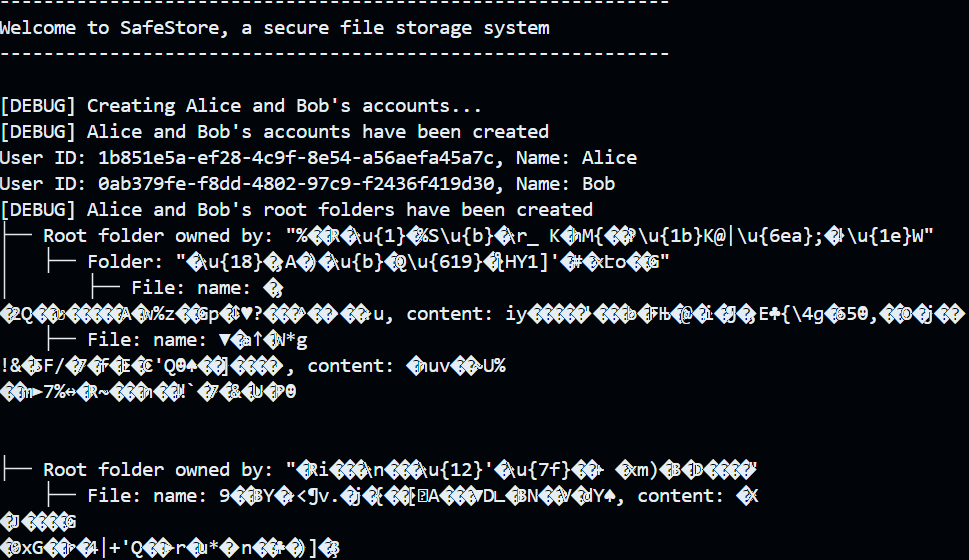
\includegraphics[width=\textwidth]{screenshots/create_procedure.png}
    \caption{Account creation procedure}
    \label{fig:create_procedure}
\end{figure}

It is important to note that the server's contents are all encrypted and this is why we see these bizarre character chains in \autoref{fig:create_procedure}. We are trying to print encrypted data to the console.


\subsubsection{Login procedure}
To decrypt the root folders we must first login as Alice. We can then decrypt her root folder:

\begin{figure}[H]
    \centering
    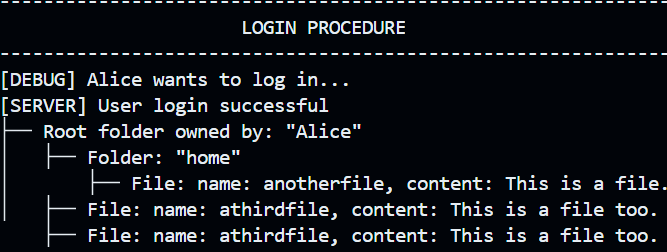
\includegraphics[width=\textwidth]{screenshots/login_procedure.png}
    \caption{Login procedure}
    \label{fig:login_procedure}
\end{figure}

As we can see in \autoref{fig:login_procedure}, Alice's root folder was decrypted. This happens client side so the server will not get any information.

\subsubsection{Password change procedure}
Alice is now logged in and she may change her password. To do this she first creates a new password, calculates a new corresponding password hash and challenge hash. She gives the challenge hash and the new password salt to the server for safekeeping. In addition to the new values, she \textbf{must} provide the same "old" challenge hash she used to login because the logout procedure with password change will perform a similar authenticity process as the login procedure. If it didn't perform this check, someone could potentially change her password without her being logged in. It automatically checks at each logout if those values are present. If they are, it updates its lists.

\begin{figure}[H]
    \centering
    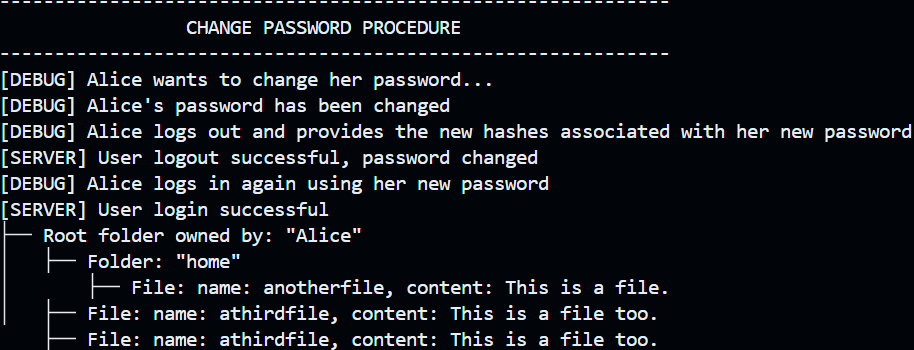
\includegraphics[width=\textwidth]{screenshots/password_procedure.png}
    \caption{Change password procedure}
    \label{fig:password_procedure}
\end{figure}

Again, all of the decryption and encryption with the new password happens client-side. The server never gets any additional information except for the new challenge hash and password salt. But alone, these are useless.

\subsubsection{Sharing folder procedure}
Alice wishes to share her "home" folder with Bob. For this, she uses Bob's public key and asymmetrically encrypts it. She then signs the hole folder. Bob receives the encrypted folder, he can verify its signature with Alice's public key as to ensure integrity of the contents. He may then decrypt it with his private key. He can then do some work on the folder.

\begin{figure}[H]
    \centering
    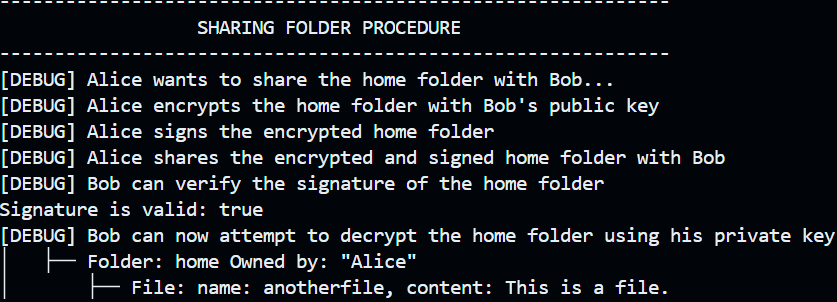
\includegraphics[width=\textwidth]{screenshots/share_procedure.png}
    \caption{Sharing folder procedure}
    \label{fig:share_procedure}
\end{figure}





\section{Discussion}
There is a lot of things that would be crucial to add but for which the time was not enough. One important thing is the fact that for now, the \lstinline{owner} field on resources is underutilized. The fact of the matter is that only in the login and logout stages authenticity is ensured but the sharing procedure does not verify ownership. This means that Bob could theoretically share any folder that Alice shares with him which is not optimal. We discussed this issue briefly in class, I think the most important aspect is trust between Alice and Bob. Mechanically, such an insurance could only be possible if Bob did not have "copyright" over the shared content. He could read it, modify it but not copy it and share it. This is a legal matter though because as long as it is made of ones and zeroes, it can be copied. Additionally, a way for Bob to be able to write the data that is being shared with him would also be interesting. This procedure was explained in previous sections. 

A big lack my framework has is the ability of interacting with it. For now it only provides tools and a brief demonstration of each implemented procedure. A real interface would have been ideal however out of scope it may be for this project.
\section{Conclusion}
The framework provides four different procedures of handling file system interactions. The main server unit will not get into contact with sensitive information. The procedures implemented and demonstrated are an account creation procedure, a login procedure, a password change procedure and finally a sharing procedure allowing two users to exchange private folders between each other. In my implementation, I cannot see a way for an attacker to get around a difficult problem and it seems that even if a total server leak occurs, unless something was not properly encrypted when it was uploaded, no data should be visible. Even a password dictionary attack would not result in any good solution, the password salt would be provided by the server for anyone but there is still the slow argon2 process to overcome before being able to test a password's validity. Again, the server would also be able to notice repeated challenge requests and block attackers accordingly, this is a well-known security measure. 


\begin{thebibliography}{9}
    \bibitem{touch}
    touch Command - Linux manual page. (n.d.). \href{https://man7.org/linux/man-pages/man1/touch.1.html}{https://man7.org/linux/man-pages/man1/touch.1.html}
\end{thebibliography}

\end{document}